\section{Hausdorffova míra a~Hausdorffova dimenze}\label{sec:hausdorffova-mira-dimenze}

Způsobů,~jak definovat dimenzi je celá řada. Zatím jsme společně prozkoumali box-counting dimenzi (resp. některá její pojetí),~avšak lze najít více způsobů její definice\footnote{Některé další jsou sepsány např. v~\citep[str. 40]{Falconer2014}.}. Pravděpodobně však nejstarším exemplářem svého druhu je tzv. \emph{Hausdorffova dimenze} a~s~ní související \emph{Hausdorffova míra},~které hrají ve fraktální geometrii velice podstatnou roli. Stále se však budeme zabývat pouze množinami v~$\R^n$. Jsou pojmenovány po německém matematikovi \name{Felixi Hausdorffovi} (1868--1942).
\begin{figure}[h]
    \centering
    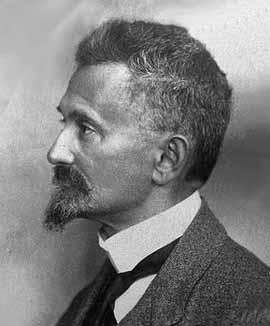
\includegraphics[width=0.4\textwidth]{felix-hausdorff.jpg}
    \caption[Felix Hausdorff,~1868--1942]{Felix Hausdorff\footnote{Převzato z~\cite{OConnorHausdorff2025}},~1868--1942}
    \label{fig:felix-hausdorff}
\end{figure}

\subsection{Definice Hausdorffovy míry}\label{subsec:hd-mira-definice}

\begin{definition}\label{def:hd-mira-delta}
    Nechť je dána množina $F\subseteq\R^n$ a~$s>0$. Pak pro každé $\delta>0$ definujeme zobrazení
    \[\hausdorffdeltameasure{s}{\delta}(F)=\inf\set{\sum_{i=1}^{\infty}(\diam{F_i})^s\;\middle|\;F\subseteq\bigcup_{i=1}^\infty F_i\;,\;\diam{F_j}\leqslant\delta\;\text{pro}\;j\in\N}.\]
\end{definition}
Na první pohled si lze všimnout,~že pro $0<\delta_1<\delta_2$ je $\hausdorffdeltameasure{s}{\delta_1}(F)\geqslant\hausdorffdeltameasure{s}{\delta_2}(F)$. Jinými slovy,~funkce $\delta\mapsto\hausdorffdeltameasure{s}{\delta}(M)$ je nerostoucí. Toto není nikterak těžké si rozmyslet,~neboť pro $\delta_1<\delta_2$ existuje $\delta_1$-pokrytí $\mathcal{F}_1$,~takové,~že je podpokrytím $\delta_2$-pokrytí $\mathcal{F}_2$ množiny $F$,~tedy $\mathcal{F}_1\subseteq\mathcal{F}_2$. To znamená,~že
\begin{align*}
    \hausdorffdeltameasure{s}{\delta_1}(F)&=\inf\set{\sum_{U\in\mathcal{F}_1}(\diam{U})^s\;\middle|\;\text{$\mathcal{F}_1$ je $\delta_1$-pokrytí $\mathcal{F}$}}\\
    &\geqslant\inf\set{\sum_{U\in\mathcal{F}_2}(\diam{U})^s\;\middle|\;\text{$\mathcal{F}_2$ je $\delta_2$-pokrytí $\mathcal{F}$}}=\hausdorffdeltameasure{s}{\delta_2}(F).
\end{align*}
Zároveň je z~definice~\ref{def:hd-mira-delta} zjevné,~že $\mathcal{H}_\delta^s(F)\geqslant 0$.
\begin{definition}[Hausdorffova míra]\label{def:hausdorffova-mira}
    Nechť $F\subseteq\R^n$. Pak pro množinu $F$ definujeme \emph{$s$-dimenzionální Hausdorffovu míru}\index{míra!Hausdorffova}\index{Hausdorffova míra} jako
    \[\hausdorffmeasure{s}(F)=\lim_{\delta\to 0}\hausdorffdeltameasure{s}{\delta}(F).\]
\end{definition}
Z přechodzího je zjevné,~že limita v~definici~\ref{def:hausdorffova-mira} vždy existuje.

Bude dobré se přesvědčit,~že je Hausdorffova míra mírou ve smyslu definice~\ref{def:prostor-s-mirou}. Začneme však otázkou. \emph{Na jaké množině je potřeba Hausdorffovu míru $\hausdorffmeasure{s}$ uvažovat?} Odpověď nám poskytují tzv. \emph{borelovské množiny}\index{množina!borelovská}\index{borelovská množina},~které jsou pojmenovány po francouzském matematikovi \name{Émile Borelovi} (1871--1956).
\begin{figure}[h]
    \centering
    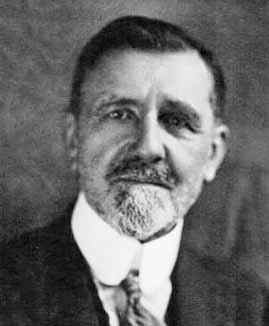
\includegraphics[width=0.4\textwidth]{Emile-Borel.jpeg}
    \caption[Émile Borel,~1871--1956]{Émile Borel\footnote{Převzato z~\cite{OConnorBorel2025}},~1871--1956}
    \label{fig:emile-borel}
\end{figure}
Borelovské množiny hrají podstatnou roli v~tzv. \emph{Deskriptivní teorii množin}. Nebudeme si zde vykládat všechny souvislosti,~vystačíme si se základem. Takto nazýváme všechny množiny,~které lze získat iteracemi operacemi spočetného sjednocení,~průniku a~doplňku otevřených množin z~$X$. Označme systém takových množin jako $\mathcal{G}$. Na tomto základě pak definujeme tzv. \emph{$\sigma$-algebru borelovských množin na $X$}:
\[\borelsigmaalgebra(X)=\bigcap_{\substack{\mathcal{F}\supseteq\mathcal{G}\\\text{$\mathcal{F}$ je $\sigma$-algebra}}}\mathcal{F}.\]
Jinými slovy,~$\borelsigmaalgebra(X)$ je nejmenší $\sigma$-algebra generovaná\footnote{Obecně $\sigma$-algebra $\mathcal{A}$ je generovaná množinou $X$,~když
\[\mathcal{A}=\bigcap_{\substack{\mathcal{F}\supseteq X\\\text{$\mathcal{F}$ je $\sigma$-algebra}}}\mathcal{F}.\]
Tento fakt se někdy značí $\mathcal{A}=\sigma(X)$.} všemi otevřenými množinami z~$X$.

Nás speciálně bude zajímat $\sigma$-algebra $\borelsigmaalgebra(\R^n)$. Nejdříve si však dokážeme dvě pomocná lemmata.
\begin{lemma}[$\sigma$-subaditivita Hausdorffovy míry]\label{lem:Hausdorffova-mira-subaditivita}
    Nechť jsou dány množiny $A_1,A_2,\ldots$,~kde $A_i\subseteq X$ pro každé $i\in\N$. Pak pro každé $s\geqslant 0$ platí
    \[\hausdorffmeasure{s}\left(\bigcup_{i=1}^\infty A_i\right)\leqslant\sum_{i=1}^{\infty}\hausdorffmeasure{s}(A_i).\]
\end{lemma}
\begin{proof}
    Nechť $s\geqslant 0$ a~dále budiž dáno $\varepsilon>0$. Pro každé $i\in\N$ a~$\delta>0$ mějme pokrytí
    \[\mathcal{F}_i=\set{F_{i,1},F_{i,2},\dots}\]
    množiny $A_i$,~takové,~že platí
    \[\sum_{j=1}^{\infty}(\diam{F_{i,j}})^s\leqslant\hausdorffdeltameasure{s}{\delta}(A_i)+\dfrac{\varepsilon}{2^i}.\]
    Systém $\bigcup_{i=1}^\infty\mathcal{F}_i$ tedy tvoří $\delta$-pokrytí množiny $A=\bigcup_{i=1}^\infty A_i$. Celkově
    \begin{align*}
        \hausdorffdeltameasure{s}{\delta}\left(\bigcup_{i=1}^\infty A_i\right)&\leqslant\sum_{i,j\in\N}(\diam{F_{i,j}})^s=\sum_{i=1}^{\infty}\sum_{j=1}^{\infty}(\diam{F_{i,j}})^s\leqslant\sum_{i=1}^{\infty}\left(\hausdorffdeltameasure{s}{\delta}(A_i)+\dfrac{\varepsilon}{2^i}\right)\\
        &=\sum_{i=1}^{\infty}\hausdorffdeltameasure{s}{\delta}(A_i)+\varepsilon.
    \end{align*}
    Limitním přechodem $\delta\to 0$ a~aplikací Leviho věty\footnote{\emph{Leviho věta o~záměně pořadí limity a~Lebesgueova integrálu} říká,~že je-li posloupnost nezáporných měřitelných funkcí $\set{f_n}_{n=1}^\infty$ neklesající,~tj.
    \[f_1\leqslant f_2\leqslant\dots\]
    na prostoru $(X,\mathcal{A},\mu)$ a~zároveň $\lim_{n\to\infty}f_n(x)=f(x)$ pro každé $x\in X$,~pak
    \[\lim_{n\to\infty}\int_X f_n\dx[\mu]=\int_X \lim_{n\to\infty}f_n\dx[\mu].\]
    Zde je speciálně $\mu$ aritmetická míra,~$X=\N$,~a $f_n(i)$ lze volit např. $\hausdorffdeltameasure{s}{1/n}(A_i)$. Z~Heineho věty víme,~že
    \[\lim_{n\to\infty}\hausdorffdeltameasure{s}{1/n}(A_i)=\lim_{\delta\to 0}\hausdorffdeltameasure{s}{\delta}(A_i)=\hausdorffmeasure{s}(A_i).\]
    }
    dostáváme
    \begin{align*}
        \hausdorffmeasure{s}\left(\bigcup_{i=1}^\infty A_i\right)&=\lim_{\delta\to 0}\hausdorffdeltameasure{s}{\delta}\left(\bigcup_{i=1}^\infty A_i\right)\leqslant\lim_{\delta\to 0}\sum_{i=1}^{\infty}\hausdorffdeltameasure{s}{\delta}(A_i)+\varepsilon=\sum_{i=1}^{\infty}\lim_{\delta\to 0}\hausdorffdeltameasure{s}{\delta}(A_i)+\varepsilon\\
        &=\sum_{i=1}^{\infty}\hausdorffmeasure{s}(A_i)+\varepsilon.
    \end{align*} 
\end{proof}
\begin{lemma}\label{lem:hausdorffova-mira-sigma-aditivita-kladna-vzdalenost}
    Nechť $(X,\varrho)$ je metrický prostor,~kde $X\subseteq\R^n$,~a $A,B\subseteq X$,~takové,~že pro jejich vzdálenost platí $\varrho(A,B)>0$. Pak pro každé $s\geqslant 0$ platí
    \[\hausdorffmeasure{s}(A\cup B)=\hausdorffmeasure{s}(A)+\hausdorffmeasure{s}(B).\]
\end{lemma}
\begin{proof}
    Nerovnost $\hausdorffmeasure{s}(A\cup B)\leqslant\hausdorffmeasure{s}(A)+\hausdorffmeasure{s}(B)$ je zřejmá ze $\sigma$-subaditivity Hausdorffovy míry (viz lemma~\ref{lem:Hausdorffova-mira-subaditivita}).

    Bez újmy na obecnosti předpokládejme,~že $\hausdorffmeasure{s}(A\cup B)<\infty$. Mějme libovolné $\varepsilon>0$. Zvolme $\delta$-pokrytí $\mathcal{F}=\set{F_1,F_2,\ldots}$ množiny $A\cup B$,~takové,~že
    \[\sum_{i=1}^{\infty}(\diam{F_i})^s\leqslant\hausdorffdeltameasure{s}{\delta}(A\cup B)+\varepsilon.\]
    Opět bez újmy na obecnosti lze předpokládat,~že pro každé $i\in\N$ je $\diam{F_i}<\varrho(A,B)$. V~opačném případě bychom $F_i$ pokryli množnami s~menším průměrem. Z~toho pak plyne,~že každá z~množin $F_i$ má neprázdný průnik s~nejvýše jednou z~množin $A,B$,~tzn. z~pokrytí $\mathcal{F}$ lze vybrat dva disjunktní podsystémy $\mathcal{F}_A$ a~$\mathcal{F}_B$,~přičemž $\bigcup\mathcal{F}_A\supseteq A$ a~$\bigcup\mathcal{F}_B\supseteq B$. Tedy celkově s~užitím předchozího lemmatu~\ref{lem:Hausdorffova-mira-subaditivita} máme
    \begin{align*}
        \hausdorffdeltameasure{s}{\delta}(A)+\hausdorffdeltameasure{s}{\delta}(B)&\leqslant\hausdorffdeltameasure{s}{\delta}\left(\bigcup_{F\in\mathcal{F}_A}F\right)+\hausdorffdeltameasure{s}{\delta}\left(\bigcup_{F\in\mathcal{F}_B}F\right)\\
        &\leqslant\sum_{F\in\mathcal{F}_A}(\diam{F})^s+\sum_{F\in\mathcal{F}_B}(\diam{F})^s\\
        &\leqslant\sum_{i=1}^{\infty}(\diam{F_i})^s\leqslant\hausdorffdeltameasure{s}{\delta}(A\cup B)+\varepsilon.
    \end{align*}
    Pro $\delta\to 0$ dostáváme
    \[\hausdorffmeasure{s}(A)+\hausdorffmeasure{s}(B)\leqslant\hausdorffmeasure{s}(A\cup B)+\varepsilon\]
\end{proof}

\begin{definition}[Vnější míra]\label{def:vnejsi-mira}
    Nechť $(X,\mathcal{A})$ je měřitelný prostor. Zobrazení $\mapping{\mu^*}{\mathcal{A}}{\langle0,\infty\rangle}$ nazveme \emph{vnější mírou}\index{míra!vnější}\index{vnější míra} na $\mathcal{A}$,~pokud platí:
    \begin{enumerate}[label=(\alph*)]
        \item\label{def:vnejsi-mira-prazdna-mnozina} $\mu^*(\emptyset)=0$,
        \item\label{def:vnejsi-mira-monotonie} Pokud $A,B\in\mathcal{A}$ a~$A\subseteq B$,~pak $\mu^*(A)\leqslant\mu^*(B)$.
        \item\label{def:vnejsi-mira-sigma-subaditivita} Je-li $A_1,A_2,\ldots$ posloupnost množin,~kde $A_i\in\mathcal{A}$ pro každé $i\in\N$,~pak
        \[\mu^*\left(\bigcup_{i=1}^\infty A_i\right)\leqslant\sum_{i=1}^{\infty}\mu^*(A_i).\]
    \end{enumerate}
\end{definition}

Vnější míra představuje zobecnění toho,~co jsme měli možnost vidět již v~sekci~\ref{sec:lebesgueova-mira} týkající Lebesgueovy míry\footnote{Jedná se slabší požadavek,~tzn. každá míra je vnější mírou,~opačné tvrzení však neplatí.}. Tu jsme definovali na základě tzv. \emph{vnější Lebesgueovy míry} (viz definice~\ref{def:vnejsi-lebegueova-mira}),~která sice sama o~sobě míru nepředstavovala,~nicméně při restrikci na "správný" systém množin jsme konstatovali,~že se již jedná o~míru. Lze se přesvědčit,~že vnější Lebesgueova míra $\lebesgueoutermeasure{n}$ je vnější mírou ve smyslu definice~\ref{def:vnejsi-mira} výše. Podobné pozorování lze učinit i~pro Hausdorffovu míru $\hausdorffmeasure{s}$. Platnost podmínky~\ref{def:vnejsi-mira-sigma-subaditivita} jsme dokázali v~lemmatu~\ref{lem:Hausdorffova-mira-subaditivita} a~o platnosti~\ref{def:vnejsi-mira-prazdna-mnozina} a~\ref{def:vnejsi-mira-monotonie} se může čtenář velice snadno předvědčit. Tedy Hausdorffova míra na měřitelném prostoru $(X,\mathcal{A})$ je vnější mírou. Navíc pokud vnější míra $\mu^*$ splňuje závěr lemmatu~\ref{lem:hausdorffova-mira-sigma-aditivita-kladna-vzdalenost},~pak ji nazýváme \emph{metrickou vnější mírou}\index{míra!metrická}\index{metrická míra}.

Carathéodoryho kritérium,~které jsme si uváděli při zavádění \emph{lebesgueovské měřitelnosti}\index{měřitelnost!lebesgueovská}\index{lebesgueovská měřitelnost} (viz definice~\ref{def:lebesgueovska-meritelnost}). Ta jednoduše říkala,~že rozdělením libovolné množiny $G$ pomocí pěvně zvolené množiny $A$ lze stanovit její míru jako součet měr dílčích částí,~tzn. $G\cap A$ a~$G\setminus A$. Tento koncept lze však rozšířit. Obecně jakákoliv množina je $\mu$-měřitelná,~pokud splňuje Carathéodoryho kritérium.
\begin{definition}\label{def:meritelnost}
    Nechť $\mu$ je míra a~$A\subseteq X$. Množina $A$ je $\mu$-měřitelná,~pokud pro každé $G\subseteq X$ platí
    \[\mu(G)=\mu(G\cap A)+\mu(G\setminus A).\]
\end{definition}
Speciálně nyní ukážeme platnost následujícího tvrzení~\ref{thm:hs-meritelnost-borel-mnozin}.
\begin{theorem}\label{thm:hs-meritelnost-borel-mnozin}
    Nechť $(X,\varrho)$ je metrický prostor. Pak každá množina $A\in\borelsigmaalgebra(X)$ je $\hausdorffmeasure{s}$-měřitelná pro každé $s\geqslant 0$.
\end{theorem}
\begin{proof}
    Není těžké si rozmyslet,~že $\borelsigmaalgebra(X)$ vyjma otevřených množin obsahuje též všechny uzavřené\footnote{Plyne z~uzavřenosti na doplněk.}. Volme tedy uzavřenou množinu $A\in\borelsigmaalgebra(X)$,~$G\subseteq X$ a~$s\geqslant 0$. Ze $\sigma$-subaditivity plyne nerovnost
    \[\hausdorffmeasure{s}(G)\leqslant\hausdorffmeasure{s}(G\cap A)+\hausdorffmeasure{s}(G\setminus A).\]
    Pro důkaz opačné nerovnosti definujeme posloupnost množin $P_0,P_1,P_2,\ldots$ následovně:
    \begin{align*}
        P_0&=\set{x\in G\mid\varrho(x,A)\geqslant 1},\\
        P_i&=\set{x\in G\;\middle|\;\dfrac{1}{i+1}\leqslant\varrho(x,A)\leqslant\dfrac{1}{i}}\;,\;i\geqslant 1.
    \end{align*}
    Pro libovolnou dvojici množin z~podposloupnosti $P_0,P_2,P_4,\ldots$ platí,~že jejich vzdálenosti jsou kladné. Z~faktu,~že $\hausdorffmeasure{s}$ je metrická (viz lemma~\ref{lem:hausdorffova-mira-sigma-aditivita-kladna-vzdalenost}) a~monotonie plyne
    \[\sum_{i=1}^{m}\hausdorffmeasure{s}(P_{2i})=\hausdorffmeasure{s}\left(\bigcup_{i=0}^m P_{2i}\right)\leqslant\hausdorffmeasure{s}(G)\]
    pro všechna $m\in\N$. Podobně pro liché členy $\sum_{i=0}^{m}\hausdorffmeasure{s}(P_{2i+1})\leqslant\hausdorffmeasure{s}(G)$. Tzn.~řada $\sum_{i=0}^{\infty}\hausdorffmeasure{s}(P_i)$ je konvergentní. Zároveň platí
    \[\varrho\left(\bigcup_{i=0}^m P_i,G\cap A\right)>0,\]
    pro každé $m\in\N$,~tedy lze psát
    \begin{align*}
        \hausdorffmeasure{s}(G\setminus A)&\leqslant\hausdorffmeasure{s}\left(\bigcup_{i=0}^m P_i\right)+\hausdorffmeasure{s}\left(\bigcup_{i=m+1}^\infty P_i\right)\\
        &\leqslant\hausdorffmeasure{s}(G)-\hausdorffmeasure{s}(G\cap A)+\sum_{i=m+1}^{\infty}\hausdorffmeasure{s}(P_i).
    \end{align*}
    Pro $m\to\infty$ dostáváme
    \[\hausdorffmeasure{s}(G\setminus A)\leqslant\hausdorffmeasure{s}(G)-\hausdorffmeasure{s}(G\cap A)\]
    z~čehož již plyne požadovaná nerovnost.
\end{proof}
\begin{corollary}\label{cor:hausdorffova-mira-je-mira}
    Trojice $(X,\borelsigmaalgebra(X),\hausdorffmeasure{s})$,~kde $X$ je libovolná množina a~$s\geqslant 0$,~tvoří prostor s~mírou.
\end{corollary}

Nyní již můžeme zobrazení $\hausdorffmeasure{s}$ nazývat mírou oprávněně. Pojďme se podívat na nějaké příklady.
\begin{example}
    Pro $s=0$ představuje zobrazení $\hausdorffmeasure{s}$ obyčejnou aritmetickou míru\index{míra!aritmetická}\index{aritmetická míra},~tzn. pro konečnou množinu $A\subseteq\R^n$ je $\hausdorffmeasure{0}(A)=|A|$. Toto není těžké ukázat. Mějme množinu $A=\set{x_1,x_2,\ldots,x_n}$. Zvolíme-li
    \[\delta<\dfrac{1}{2}\cdot\min\set{\varrho_e(x_i,x_j)\mid 1\leqslant i,j\leqslant n},\]
    pak pro $\delta$-pokrytí $\mathcal{F}=\set{F_1,F_2,\ldots,F_n}$ takové,~že $x_i\in F_i$ pro každé $i$ máme
    \[\sum_{i=1}^{n}(\diam{F_i})^0=\sum_{i=1}^{n}1=n.\]
    Není těžké si rozmyslet,~že $n$ je nejmenší počet množin o~průměru nejvýše $\delta$,~takových,~aby pokrývaly množinu $A$. Zároveň pro libovolné $\varepsilon>0$ je potřeba nejvýše $n$-koulí o~poloměru $\varepsilon/2$ se středy v~$x_i$ pro pokrytí $A$. Tzn.~$\hausdorffmeasure{0}(A)=|A|=n$.
\end{example}

V rámci tohoto textu jsme se již zabývali jiným typem míry a~to tzv. \emph{lebesgueovou mírou} (viz sekce~\ref{sec:lebesgueova-mira}). Ta pro nás hrála důležitou roli v~jednom možném pojetí \emph{box-counting dimenze} (viz sekce~\ref{sec:box-counting-dimenze}). Lze ukázat,~že pro množinu $F\subseteq\R^n$ je
\[\hausdorffmeasure{n}(F)=\dfrac{1}{v_n}\lebesguemeasure{n}(F),\]
kde $v_n$ je objem (míra) jednotkové koule v~$\R^n$. Čtenář snad promine,~že tento fakt zde ponecháme bez důkazu. \citep[str. 45]{Falconer2014}

\subsection{Stručně k~vlastnostem Hausdorffovy míry}\label{subsec:vlastnosti-hausdorffovy-miry}

Na chvíli se ještě zastavíme u~vlastností Hausdorffovy míry. Již jsme společně dokázali,~že Hausdorffova míra je skutečně mírou,~tzn. splňuje všechny základní vlastnosti,~které jsme si představili ve větě~\ref{thm:mira-vlastnosti} (viz sekce~\ref{sec:prostory-s-mirou}). V~tomto ohledu tedy netřeba již nic dalšího dokazovat. Nicméně podobně jako v~případě \emph{box-counting dimenze} (viz podsekce~\ref{subsec:vlastnosti-bc-dimenze}) se i~zde podíváme,~jak se Hausdorffova míra chová vůči \emph{lipschitzovským zobrazením}\index{zobrazení!lipschitzovské}\index{lipschitzovské zobrazení}.
\begin{theorem}\label{thm:hd-dimenze-lipschitzovske-zobrazeni}
    Nechť $F\subseteq\R^n$ v~metrickém prostoru $(\R^n,\varrho)$ a~zobrazení $\mapping{f}{F}{\R^n}$ je lipschitzovské\footnote{Tvrzení lze zformulovat obecněji pro tzv. \emph{hölderovská zobrazení}\index{zobrazení!hölderovské}\index{hölderovské zobrazení},~tedy zobrazení $f$ splnující
    \[\varrho(f(x),f(y))\leqslant K(\varrho(x,y))^\alpha.\]
    kde $\alpha>0$. Pak pro $F\subseteq\R^n$ platí
    \[\hausdorffmeasure{s/\alpha}(f(F))\leqslant K^{s/\alpha}\hausdorffmeasure{s}(F).\]
    My si však vystačíme se speciálním případem.} s~konstantou $K>0$. Pak pro každé $s\geqslant 0$ platí
    \[\hausdorffmeasure{s}(f(F))\leqslant K^s\hausdorffmeasure{s}(F).\]
\end{theorem}
\begin{proof}
    Nechť $\mathcal{F}=\set{F_1,F_2,\ldots}$ je $\delta$-pokrytí $F$. Pak
    \[\diam(f(F\cap F_i))\leqslant K\diam(F\cap F_i)\leqslant K\diam{F_i},\]
    což znamená,~že $\mathcal{G}=\set{F\cap F_1,F\cap F_2,\ldots}$ je $K\delta$-pokrytí $f(F)$. Z~toho plyne,~že
    \[\sum_{i=1}^{\infty}(\diam(f(F\cap F_i)))^s\leqslant K^s\sum_{i=1}^{\infty}(\diam{F_i})^s\]
    a~tedy $\hausdorffdeltameasure{s}{K\delta}(f(F))\leqslant K^s\hausdorffdeltameasure{s}{\delta}(F)$. Pro $\delta\to 0$ máme požadovaný výsledek.
\end{proof}
(Převzato z~\citep[str. 46]{Falconer2014}.)

Z toho speciálně plyne důsledek týkající se podobností.
\begin{corollary}\label{cor:hd-dimenze-podobnost}
    Nechť $F\subseteq\R^n$ v~metrickém prostoru $(\R^n,\varrho)$ a~zobrazení $\mapping{f}{F}{\R^n}$ je podobnost\index{podobnost},~tzn. existuje $K>0$ takové,~že pro každé $x,y\in F$ platí
    \[\varrho(f(x),f(y))=K\varrho(x,y).\]
    Pak pro každé $s\geqslant 0$ platí
    \[\hausdorffmeasure{s}(f(F))=K^s\hausdorffmeasure{s}(F).\]
\end{corollary}
\begin{proof}
    K~podobnosti $f$ existuje inverzní zobrazení $f^{-1}$ s~koeficientem $L=1/K$. Z~věty~\ref{thm:hd-dimenze-lipschitzovske-zobrazeni} tedy plyne,~že
    \[\hausdorffmeasure{s}(F)=\hausdorffmeasure{s}(f^{-1}(f(F)))\leqslant\dfrac{1}{K^s}\hausdorffmeasure{s}(f(F))\]
    nebo-li $\hausdorffmeasure{s}(f(F))\geqslant K^s\hausdorffmeasure{s}(F)$. Opačnou nerovnost získáme aplikací věty~\ref{thm:hd-dimenze-lipschitzovske-zobrazeni} na zobrazení $f$.
\end{proof}

\subsection{Hausdorffova dimenze}\label{subsec:hausdorffova-dimenze}

Středobodem této sekce je tzv. \emph{Hausdorffova dimenze}\index{dimenze!Hausdorffova}\index{Hausdorffova dimenze}. Na úvod si dokážeme jedno jednoduché tvrzení týkající se Hausdorffovy míry.
\begin{theorem}\label{thm:hodnoty-hausdorffovy-miry}
    Nechť $0\leqslant s<t<\infty$ a~$F\subseteq X$. Pak platí:
    \begin{enumerate}[label=(\roman*)]
        \item\label{thm:hd-dimenze-konecna} $\hausdorffmeasure{s}(F)<\infty\implies\hausdorffmeasure{t}(F)=0$,
        \item\label{thm:hd-dimenze-nekonecno} $\hausdorffmeasure{t}(F)>0\implies\hausdorffmeasure{s}(F)=\infty$.
    \end{enumerate}
\end{theorem}
\begin{proof}
    Mějme $\delta$-pokrytí $\mathcal{F}=\set{F_1,F_2,\ldots}$,~takové,~že
    \[\sum_{i=1}^{\infty}(\diam{F_i})^s\leqslant\hausdorffdeltameasure{s}{\delta}(F)+\varepsilon\;,\;\varepsilon>0.\]
    Pak
    \[\hausdorffdeltameasure{t}{\delta}(F)\leqslant\sum_{i=1}^{\infty}(\diam{F_i})^t\leqslant\delta^{t-s}\sum_{i=1}^{\infty}(\diam{F_i})^s\leqslant\delta^{t-s}(\hausdorffdeltameasure{s}{\delta}(F)+\varepsilon).\]
    Tzn.~$\hausdorffdeltameasure{t}{\delta}(F)\leqslant\delta^{t-s}\hausdorffdeltameasure{s}{\delta}(F)$. Pro $\delta\to 0$ dostaneme body~\ref{thm:hd-dimenze-konecna} a~\ref{thm:hd-dimenze-nekonecno}.
\end{proof}
(Převzato z~\citep[str. 68]{Mattila1995}.)

Z věty~\ref{thm:hodnoty-hausdorffovy-miry} lze vidět,~že Hausdorffova míra dává smysl jen pro určitou hodnotu $s$. Pro "příliš velké" $s$ bude hodnota vždy $0$,~naopak pro "moc malé" $s$ bude jeho hodnota rovna $\infty$ (viz obrázek~\ref{fig:hausdorffova-dimenze-graf}).
\begin{figure}[h]
    \centering
    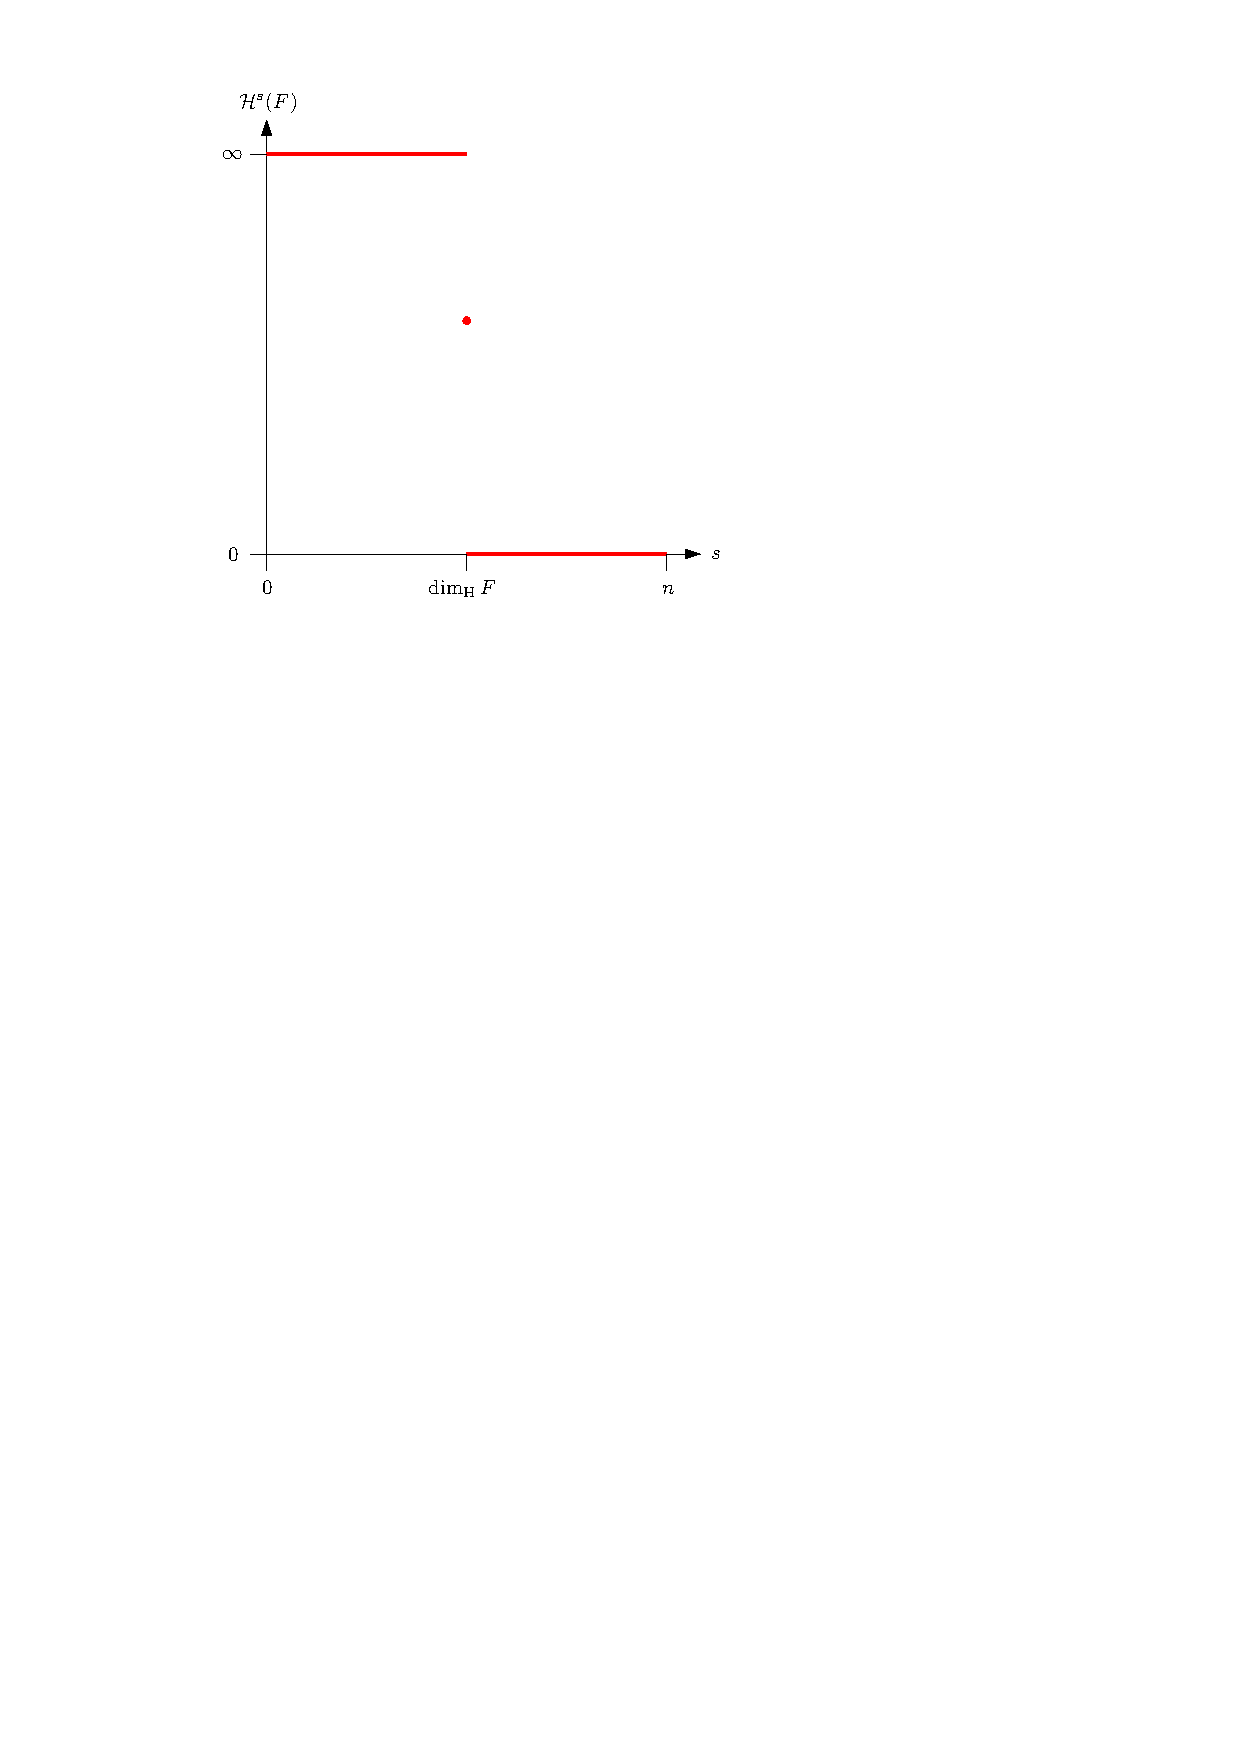
\includegraphics{ch02-hausdorffova-dimenze-graf.pdf}
    \caption{Graf funkce $f(s)=\hausdorffmeasure{s}(F)$,~kde $F\subseteq\R^n$.}
    \label{fig:hausdorffova-dimenze-graf}
\end{figure}
Této kritické hodnotě $s$ říkáme \emph{Hausdorffova dimenze}\index{dimenze!Hausdorffova}\index{Hausdorffova dimenze}.
\begin{definition}[Hausdorffova dimenze]\label{def:hausdorffova-dimenze}
    Nechť $F\subseteq\R^n$. Hausdorffovou dimenzí\footnote{Též někdy nazývaná \emph{Hausdorffova-Bezikovičova dimenze}\index{dimenze!Hausdorffova-Bezikovičkova}. }\index{dimenze!Hausdorffova}\index{Hausdorffova dimenze} množiny $F$ nazveme hodnotu
    \[\dimH{F}=\inf\set{s\geqslant 0\mid\hausdorffmeasure{s}(F)=0}=\sup\set{s\geqslant 0\mid\hausdorffmeasure{s}(F)=\infty}.\]
\end{definition}
Hodnota $\hausdorffmeasure{s}(F)$ pro $s=\dimH{F}$ může být různá,~tzn. může platit,~že $\hausdorffmeasure{s}(F)=\infty$,~$\hausdorffmeasure{s}(F)=0$ a~nebo se může jednat o~konečné nenulové číslo,~tj. $0<\hausdorffmeasure{s}(F)<\infty$.

Nyní se podívejme na příklad výpočtu. Podobně,~jako v~případě box-counting dimenze,~i zde budeme nezávisle určovat horní a~dolní odhad.
\begin{example}[Sierpińského trojúhelník]\label{ex:sierpinskeho-trojuhelnik-hd-dimenze}
    V~tomto případě se podíváme na dvě možnosti,~jak dojít k~výsledku. Celý Sierpińského trojúhelník si označme $S$.
    \begin{itemize}
        \item V~$k$-té iteraci,~kde $k=0,1,2,\ldots$,~vzniknou 3 nové trojúhelníky o~obsahu $1/4$ obsahu původního trojúhelníka,~tzn. jejich celkový počet je $t=3^k$. Uvažíme-li $\delta$-pokrytí
        \[\mathcal{K}=\set{K_\delta^1(x_1),K_\delta^2(x_2),\ldots,K_\delta^t(x_t),\emptyset,\emptyset,\ldots}\]
        kde $x_1,x_2,\ldots,x_t\in S_k$ a~$\delta\leqslant 2^{-k}/2=2^{-k-1}$,~pak
        \[\hausdorffdeltameasure{s}{2^{-k}}(S_k)\leqslant\sum_{i=1}^{3^k}(2^{-k})^s=3^k2^{-ks}=1.\]
        Pro $k\to\infty$ je $\hausdorffmeasure{s}(S)\leqslant 1$. Poslední rovnost nastává právě pro $s=\ln{3}/\ln{2}$.

        Nyní ukážeme,~že $\hausdorffmeasure{s}(S)\geqslant 3^{-s}=1/2$. Zvolme $\delta$-pokrytí
        \[\mathcal{F}=\set{F_1,F_2,\ldots},\]
        takové,~že
        \begin{equation}\label{eq:volba-delta-pokryti-F}
            2^{-k-1}\leqslant\diam{F_i}<2^{-k},
        \end{equation}
        kde $i\in\N$. Lze si rozmyslet,~že každá z~množin $F_i$ má neprázdný průnik s~nejvýše dvěma dílčími trojúhelníky. Zvolíme-li $j\geqslant k$,~pak každá z~množin $F_i$ má průnik maximálně s~$3^{j-k}$ trojúhelníky v~$j$-té iteraci,~resp.
        \[3^{j-k}=3^j2^{-ks}\leqslant2^j3^s(\diam{F_i})^s,\]
        jak plyne z~volby pokrytí $\mathcal{F}$ v~\eqref{eq:volba-delta-pokryti-F}. Pokud navíc pro každé $i\in\N$ platí,~že
        \[3^{-j-1}\leqslant\diam{F_i},\]
        pak každá z~množin $F_i$ má neprázdný průnik s~nejvýše $3^j$ trojúhelníky. Tedy pro jejich počet platí
        \[3^j\leqslant\sum_{i=1}^{\infty}3^j3^s(\diam{F_i})^s,\]
        přičemž úpravou už získáme požadovanou nerovnost.
        \item Druhá varianta výpočtu je sice méně rigorózní,~avšak podstatně jednodušší. Sierpińského trojúhelník sestává ze tří kopií sebe samotného,~přičemž každá z~nich je obrazem původního obrazce $S$ v~podobnosti s~koeficientem $K=1/2$. Označme si dané části $S_1,S_2$ a~$S_3$,~tj. $S=S_1\cup S_2\cup S_3$. Tedy podle $\sigma$-aditivity Hausdorffovy míry a~důsledku~\ref{cor:hd-dimenze-podobnost} můžeme psát
        \begin{align*}
            \hausdorffmeasure{s}(S)&=\hausdorffmeasure{s}(S_1)+\hausdorffmeasure{s}(S_2)+\hausdorffmeasure{s}(S_3)\\
            &=\left(\dfrac{1}{2}\right)^s\hausdorffmeasure{s}(S)+\left(\dfrac{1}{2}\right)^s\hausdorffmeasure{s}(S)+\left(\dfrac{1}{2}\right)^s\hausdorffmeasure{s}(S)\\
            &=3\left(\dfrac{1}{2}\right)^s\hausdorffmeasure{s}(S).
        \end{align*}
        Budeme-li předpokládat,~že $\hausdorffmeasure{s}(S)<\infty$ (jak jsme již viděli z~předchozího výpočtu,~jedná se o~netriviální předpoklad) pro $s=\dimH{S}$,~pak z~rovnosti $1=3(1/2)^s$ lze dopočítat,~že $s=\ln{3}/\ln{2}$.
    \end{itemize}
\end{example}
(Převzato a~upraveno z~\citep[str. 53]{Falconer2014}.)

Myšlenku druhého výpočtu z~příkladu~\ref{ex:sierpinskeho-trojuhelnik-hd-dimenze} ještě rozvedeme v~kapitole~\ref{chapter:klasifikace-fraktalu},~konkrétně v~sekci~\ref{sec:ifs} věnované systémům iterovaných funkcí\index{systém iterovaných funkcí}\index{systém!iterovaných funkcí}.

Jako poslední zkusme postavit Hausdorffovu dimenzi proti box-counting dimenzi představenou v~sekci~\ref{sec:box-counting-dimenze}. Vztah mezi nimi je docela jednoduchý a~udává jej věta~\ref{thm:bc-dimenze-vs-hd-dimenze}. Pro připomenutí doporučuji se opětovně podívat na definici~\ref{def:box-counting-dimenze}
\begin{theorem}\label{thm:bc-dimenze-vs-hd-dimenze}
    Nechť $F\subseteq\R^n$ je neprázdná omezená množina. Pak platí
    \[\dimH{F}\leqslant\lowerdimB{F}\leqslant\upperdimB{F}\]
\end{theorem}
\begin{proof}
    Nechť platí $1<\hausdorffmeasure{s}(F)=\lim_{\delta\to 0}\hausdorffdeltameasure{s}{\delta}(F)$ pro $s\geqslant 0$. Zvolme $\delta>0$ takové,~že platí
    \[1<\hausdorffdeltameasure{s}{\delta}(F)\leqslant N_\delta(F)\delta^s.\]
    Úpravou této nerovnosti dostaneme
    \begin{align*}
        0&<\ln{N_\delta(F)}+s\ln{\delta}\\
        s&<\dfrac{\ln{N_\delta(F)}}{-\ln{\delta}}\\
        s&\leqslant\lim_{\delta\to 0}\dfrac{\ln{N_\delta(F)}}{-\ln{\delta}}.
    \end{align*}
    Druhá nerovnost,~jak již víme,~plyne přímo z~definice box-counting dimenze (viz~\ref{def:box-counting-dimenze}). Pro případ $0<\hausdorffdeltameasure{s}{\delta}(F)<1$ stačí aplikovat podobnost na $F$ a~využít tvrzení~\ref{cor:hd-dimenze-podobnost}.
\end{proof}
(Převzato z~\citep[str. 50]{Falconer2014}.)

K závěru poznamenejme,~že mnoho "rozumných" útvarů $F$ je Hausdorffova dimenze $\dimH{F}$ rovna box-counting dimenzi $\dimB{F}$,~ale obecná rovnost zde neplatí. Např. pro množinu $X=\Q\cap\langle0,1\rangle$ je $\dimH{X}=0$,~neboť $X$ je spočetná. Nicméně v~případě box-counting dimenze je $\dimB{X}=1$. Rozmyšlení již ponecháme na čtenáři.

Pro více informací si dovolím odkázat na článek \cite{Falconer1989} věnovaný přímo této otázce.